% Options for packages loaded elsewhere
\PassOptionsToPackage{unicode}{hyperref}
\PassOptionsToPackage{hyphens}{url}
\PassOptionsToPackage{dvipsnames,svgnames,x11names}{xcolor}
%
\documentclass[
  letterpaper,
  DIV=11,
  numbers=noendperiod]{scrartcl}

\usepackage{amsmath,amssymb}
\usepackage{iftex}
\ifPDFTeX
  \usepackage[T1]{fontenc}
  \usepackage[utf8]{inputenc}
  \usepackage{textcomp} % provide euro and other symbols
\else % if luatex or xetex
  \usepackage{unicode-math}
  \defaultfontfeatures{Scale=MatchLowercase}
  \defaultfontfeatures[\rmfamily]{Ligatures=TeX,Scale=1}
\fi
\usepackage{lmodern}
\ifPDFTeX\else  
    % xetex/luatex font selection
\fi
% Use upquote if available, for straight quotes in verbatim environments
\IfFileExists{upquote.sty}{\usepackage{upquote}}{}
\IfFileExists{microtype.sty}{% use microtype if available
  \usepackage[]{microtype}
  \UseMicrotypeSet[protrusion]{basicmath} % disable protrusion for tt fonts
}{}
\makeatletter
\@ifundefined{KOMAClassName}{% if non-KOMA class
  \IfFileExists{parskip.sty}{%
    \usepackage{parskip}
  }{% else
    \setlength{\parindent}{0pt}
    \setlength{\parskip}{6pt plus 2pt minus 1pt}}
}{% if KOMA class
  \KOMAoptions{parskip=half}}
\makeatother
\usepackage{xcolor}
\setlength{\emergencystretch}{3em} % prevent overfull lines
\setcounter{secnumdepth}{-\maxdimen} % remove section numbering
% Make \paragraph and \subparagraph free-standing
\makeatletter
\ifx\paragraph\undefined\else
  \let\oldparagraph\paragraph
  \renewcommand{\paragraph}{
    \@ifstar
      \xxxParagraphStar
      \xxxParagraphNoStar
  }
  \newcommand{\xxxParagraphStar}[1]{\oldparagraph*{#1}\mbox{}}
  \newcommand{\xxxParagraphNoStar}[1]{\oldparagraph{#1}\mbox{}}
\fi
\ifx\subparagraph\undefined\else
  \let\oldsubparagraph\subparagraph
  \renewcommand{\subparagraph}{
    \@ifstar
      \xxxSubParagraphStar
      \xxxSubParagraphNoStar
  }
  \newcommand{\xxxSubParagraphStar}[1]{\oldsubparagraph*{#1}\mbox{}}
  \newcommand{\xxxSubParagraphNoStar}[1]{\oldsubparagraph{#1}\mbox{}}
\fi
\makeatother


\providecommand{\tightlist}{%
  \setlength{\itemsep}{0pt}\setlength{\parskip}{0pt}}\usepackage{longtable,booktabs,array}
\usepackage{calc} % for calculating minipage widths
% Correct order of tables after \paragraph or \subparagraph
\usepackage{etoolbox}
\makeatletter
\patchcmd\longtable{\par}{\if@noskipsec\mbox{}\fi\par}{}{}
\makeatother
% Allow footnotes in longtable head/foot
\IfFileExists{footnotehyper.sty}{\usepackage{footnotehyper}}{\usepackage{footnote}}
\makesavenoteenv{longtable}
\usepackage{graphicx}
\makeatletter
\newsavebox\pandoc@box
\newcommand*\pandocbounded[1]{% scales image to fit in text height/width
  \sbox\pandoc@box{#1}%
  \Gscale@div\@tempa{\textheight}{\dimexpr\ht\pandoc@box+\dp\pandoc@box\relax}%
  \Gscale@div\@tempb{\linewidth}{\wd\pandoc@box}%
  \ifdim\@tempb\p@<\@tempa\p@\let\@tempa\@tempb\fi% select the smaller of both
  \ifdim\@tempa\p@<\p@\scalebox{\@tempa}{\usebox\pandoc@box}%
  \else\usebox{\pandoc@box}%
  \fi%
}
% Set default figure placement to htbp
\def\fps@figure{htbp}
\makeatother

\KOMAoption{captions}{tableheading}
\makeatletter
\@ifpackageloaded{caption}{}{\usepackage{caption}}
\AtBeginDocument{%
\ifdefined\contentsname
  \renewcommand*\contentsname{Table of contents}
\else
  \newcommand\contentsname{Table of contents}
\fi
\ifdefined\listfigurename
  \renewcommand*\listfigurename{List of Figures}
\else
  \newcommand\listfigurename{List of Figures}
\fi
\ifdefined\listtablename
  \renewcommand*\listtablename{List of Tables}
\else
  \newcommand\listtablename{List of Tables}
\fi
\ifdefined\figurename
  \renewcommand*\figurename{Figure}
\else
  \newcommand\figurename{Figure}
\fi
\ifdefined\tablename
  \renewcommand*\tablename{Table}
\else
  \newcommand\tablename{Table}
\fi
}
\@ifpackageloaded{float}{}{\usepackage{float}}
\floatstyle{ruled}
\@ifundefined{c@chapter}{\newfloat{codelisting}{h}{lop}}{\newfloat{codelisting}{h}{lop}[chapter]}
\floatname{codelisting}{Listing}
\newcommand*\listoflistings{\listof{codelisting}{List of Listings}}
\makeatother
\makeatletter
\makeatother
\makeatletter
\@ifpackageloaded{caption}{}{\usepackage{caption}}
\@ifpackageloaded{subcaption}{}{\usepackage{subcaption}}
\makeatother

\usepackage{bookmark}

\IfFileExists{xurl.sty}{\usepackage{xurl}}{} % add URL line breaks if available
\urlstyle{same} % disable monospaced font for URLs
\hypersetup{
  pdftitle={Expected Utility \& Its\,Critiques},
  pdfauthor={Tilman~Fries},
  colorlinks=true,
  linkcolor={blue},
  filecolor={Maroon},
  citecolor={Blue},
  urlcolor={Blue},
  pdfcreator={LaTeX via pandoc}}


\title{Expected Utility \& Its\,Critiques}
\usepackage{etoolbox}
\makeatletter
\providecommand{\subtitle}[1]{% add subtitle to \maketitle
  \apptocmd{\@title}{\par {\large #1 \par}}{}{}
}
\makeatother
\subtitle{Expected\,Utility\,Theory, Subjective\,EUT, Probability
Weighting}
\author{Tilman~Fries}
\date{}

\begin{document}
\maketitle


\subsection{Decisions under Risk and
Uncertainty}\label{decisions-under-risk-and-uncertainty}

\begin{itemize}
\tightlist
\item
  People take many decisions daily where they do not know exactly what
  will happen.
\item
  Think about choosing when to leave house to get to this lecture.

  \begin{itemize}
  \tightlist
  \item
    Will the bus be on time?
  \item
    How much does it matter if I miss the first 5 minutes of
    class\ldots?
  \end{itemize}
\item
  This is highly a highly complex problem.
\item
  Yet we solve hundrets of them daily.
\end{itemize}

\subsection{Terminology}\label{terminology}

\begin{itemize}
\tightlist
\item
  In economics, we distinguish between decisions under {risk} and
  decisions under {uncertainty}.
\item
  Risk has known probabilities, it is a \emph{known unknown}:

  \begin{itemize}
  \tightlist
  \item
    The probability of a die roll of four.
  \item
    Winning at roulette.
  \end{itemize}
\item
  You do not know uncertain probabilities, they are an \emph{unknown
  unknown}.

  \begin{itemize}
  \tightlist
  \item
    Whether stocks will go up or down.
  \item
    The climate impact of your lunch.
  \end{itemize}
\end{itemize}

\subsection{Plan}\label{plan}

\begin{itemize}
\tightlist
\item
  Two central economic theories exist to describe how individuals behave
  under risk and uncertainty.

  \begin{itemize}
  \tightlist
  \item
    Risk: Expected Utility Theory
  \item
    Uncertainty: Subjective Expected Utility Theory
  \end{itemize}
\item
  They are central to economic modeling.
\item
  We will learn about them now.
\item
  Then we will learn about behavioral economic critiques.
\end{itemize}

\begin{center}\rule{0.5\linewidth}{0.5pt}\end{center}

\subsection{Expected~Utility~Theory
(EUT)}\label{expected-utility-theory-eut}

\begin{itemize}
\tightlist
\item
  An agent chooses between \textbf{lotteries}
  \(p\,\in\,\mathcal{P}(\mathcal{Z})\) that map outcomes
  \(z\in\mathcal{Z}\) to probabilities.

  \begin{itemize}
  \tightlist
  \item
    Example of a lottery: Flip a coin. If heads, 5€. If tails, 0€.
  \item
    We will denote this lottery as \((5, 0.5; 0, 0.5)\).
  \end{itemize}
\item
  The agent has \textbf{preferences} \(\succeq\) over lotteries.

  \begin{itemize}
  \tightlist
  \item
    Example of a preference: \((2, 1)\succeq (5, 0.5; 0, 0.5)\).
  \item
    The preferences follow certain \textbf{axioms} (next slide).
  \end{itemize}
\end{itemize}

\begin{center}\rule{0.5\linewidth}{0.5pt}\end{center}

\subsection{Axioms of~EUT}\label{axioms-of-eut}

\phantomsection\label{ax:rational}
\textbf{Rationality.} --- the usual completeness~\& transitivity.

\phantomsection\label{ax:independence}
\textbf{Independence.} If \(p \succ q\) then for any lottery \(r\) and
\(\alpha\in(0,1]\)
\[\alpha p+(1-\alpha)r \;\succ\; \alpha q+(1-\alpha)r.\]

\begin{center}\rule{0.5\linewidth}{0.5pt}\end{center}

\subsection{Axioms of~EUT}\label{axioms-of-eut-1}

\phantomsection\label{ax:independence}
\textbf{Independence.} If \(p \succ q\) then for any lottery \(r\) and
\(\alpha\in(0,1]\)
\[\alpha p+(1-\alpha)r \;\succ\; \alpha q+(1-\alpha)r.\]

\begin{itemize}
\tightlist
\item
  \(\alpha p+(1-\alpha)r\) is a \emph{compound lottery.}
\item
  E.g., \(p\) is lottery ``win 5€ if heads'' and \(r\) is lottery ``win
  10€ if die is odd''.
\item
  \(\alpha\) is a probability, e.g., 40\%.
\end{itemize}

\begin{center}\rule{0.5\linewidth}{0.5pt}\end{center}

\subsection{Axioms of~EUT}\label{axioms-of-eut-2}

\phantomsection\label{ax:independence}
\textbf{Independence.} If \(p \succ q\) then for any lottery \(r\) and
\(\alpha\in(0,1]\)
\[\alpha p+(1-\alpha)r \;\succ\; \alpha q+(1-\alpha)r.\]

\begin{itemize}
\tightlist
\item
  E.g., p is lottery ``win 5€ if heads'' and r is lottery ``win 10€ if
  die is odd''.
\item
  \(\alpha\) is a probability, e.g., 40\%.
\item
  Then, this reads as ``With 40\%, toss coin and win 5€ if heads. With
  60\%, roll die and win 10€ if odd.''
\end{itemize}

\begin{center}\rule{0.5\linewidth}{0.5pt}\end{center}

\subsection{Axioms of~EUT}\label{axioms-of-eut-3}

\phantomsection\label{ax:independence}
\textbf{Independence.} If \(p \succ q\) then for any lottery \(r\) and
\(\alpha\in(0,1]\)
\[\alpha p+(1-\alpha)r \;\succ\; \alpha q+(1-\alpha)r.\]

\begin{itemize}
\tightlist
\item
  Independence basically says that the agent focuses on the things that
  are different when comparing lotteries.

  \begin{itemize}
  \tightlist
  \item
    Both lotteries contain \((1-\alpha)r\).
  \item
    Therefore, decide only based on comparing \(p\) and \(q\) because
    they are different.
  \end{itemize}
\end{itemize}

\begin{center}\rule{0.5\linewidth}{0.5pt}\end{center}

\subsection{Axioms of~EUT}\label{axioms-of-eut-4}

\phantomsection\label{ax:continuity}
\textbf{Continuity.} If \(p\succeq q\succeq r\) and \(p\succ r\) then
there is an \(\alpha\in[0,1]\) with
\[q\;\sim\; \alpha p + (1-\alpha)r.\]

\begin{itemize}
\tightlist
\item
  The agent takes their most and least preferred lottery and can mix
  them such that agent is indifferent between the mix and any other
  lottery.
\end{itemize}

\begin{center}\rule{0.5\linewidth}{0.5pt}\end{center}

\subsection{Axioms of~EUT}\label{axioms-of-eut-5}

\phantomsection\label{ax:continuity}
\textbf{Continuity.} If \(p\succeq q\succeq r\) and \(p\succ r\) then
there is an \(\alpha\in[0,1]\) with
\[q\;\sim\; \alpha p + (1-\alpha)r.\]

\begin{itemize}
\tightlist
\item
  Sounds intuitive, but consider, e.g., your least preferred lottery
  being ``death with probability 1''. Would you mix that with anything?
\end{itemize}

\begin{center}\rule{0.5\linewidth}{0.5pt}\end{center}

\subsection{Expected Utility
Representation}\label{expected-utility-representation}

\phantomsection\label{prop:EUT}
\textbf{Proposition.} If \(\succeq\) satisfies rationality,
independence, and continuity, then there exists a utility function
\(u:\mathcal{Z}\to\mathbb{R}\) such that \[
p\succeq q \quad\Longleftrightarrow\quad \sum_{z\in\mathcal{Z}} p(z)\,u(z)\;\ge\; \sum_{z\in\mathcal{Z}} q(z)\,u(z).
\]

\begin{itemize}
\tightlist
\item
  In the EU representation, utility of an outcome scales linearly in its
  probability.
\item
  E.g., The EU of lottery \((5, \frac{1}{6}; 0, \frac{5}{6})\) is
  \(\frac{1}{6} u(5) + \frac{5}{6} u(0).\)
\end{itemize}

\begin{center}\rule{0.5\linewidth}{0.5pt}\end{center}

\subsection{Proof Sketch: EU
Representation}\label{proof-sketch-eu-representation}

\begin{itemize}
\tightlist
\item
  That EU is linear in probability is the consequence of the
  \textbf{independence} and \textbf{continuity} axioms.
\item
  Independence implies the following lemma:
\end{itemize}

\textbf{Lemma.} If \(p\succ q\) and \(0\leq \alpha < \beta \leq 1\),
then \(\beta p + (1-\beta)q\succ \alpha p + (1-\alpha)q\).

Proof on board.

\begin{center}\rule{0.5\linewidth}{0.5pt}\end{center}

\subsection{Proof Sketch: EU
Representation}\label{proof-sketch-eu-representation-1}

\begin{itemize}
\tightlist
\item
  Now take the worst possible outcome and the best possible outcome and
  put them on a utility scale (e.g., \(U(\text{Worst}) = 0\),
  \(U(\text{best}) = 1\)).
\end{itemize}

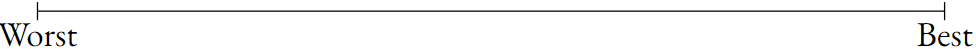
\includegraphics[width=1\linewidth,height=\textheight,keepaspectratio]{figures/WorstBestEmpty.png}

\begin{center}\rule{0.5\linewidth}{0.5pt}\end{center}

\subsection{Proof Sketch: EU
Representation}\label{proof-sketch-eu-representation-2}

\begin{itemize}
\tightlist
\item
  Now take the worst possible outcome and the best possible outcome and
  put them on a utility scale (e.g., \(U(\text{Worst}) = 0\),
  \(U(\text{best}) = 1\)).
\item
  By \textbf{continuity} there is a probability \(f(p)\) such that \[ 
  p \sim f(p)\text{Best} + (1-f(p))\text{Worst}. 
  \]
\end{itemize}

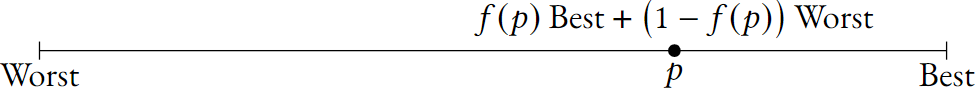
\includegraphics[width=1\linewidth,height=\textheight,keepaspectratio]{figures/WorstBestP.png}

\begin{center}\rule{0.5\linewidth}{0.5pt}\end{center}

\subsection{Proof Sketch: EU
Representation}\label{proof-sketch-eu-representation-3}

\begin{itemize}
\tightlist
\item
  Now take the worst possible outcome and the best possible outcome and
  put them on a utility scale (e.g., \(U(\text{Worst}) = 0\),
  \(U(\text{best}) = 1\)).
\item
  By \textbf{continuity} there is a probability \(f(p)\) such that \[ 
  p \sim f(p)\text{Best} + (1-f(p))\text{Worst}. 
  \]
\item
  By the lemma, if \(p\succ q\), then \(f(p) > f(q)\).
\end{itemize}

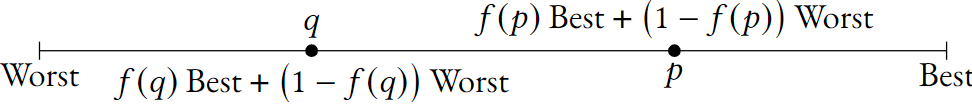
\includegraphics[width=1\linewidth,height=\textheight,keepaspectratio]{figures/WorstBestPQ.png}

\begin{center}\rule{0.5\linewidth}{0.5pt}\end{center}

\subsection{Proof Sketch: EU
Representation}\label{proof-sketch-eu-representation-4}

\begin{itemize}
\tightlist
\item
  By \textbf{continuity} there is a probability \(f(p)\) such that \[ 
  p \sim f(p)\text{Best} + (1-f(p))\text{Worst}. 
  \]
\item
  By the lemma, if \(p\succ q\), then \(f(p) > f(q)\).
\end{itemize}

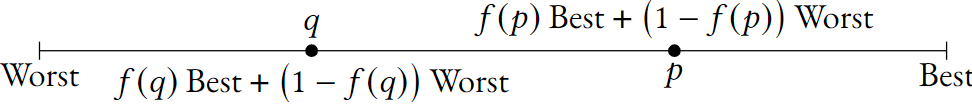
\includegraphics[width=1\linewidth,height=\textheight,keepaspectratio]{figures/WorstBestPQ.png}

\begin{itemize}
\tightlist
\item
  The full proof shows that \(f(p)\) is affine, which implies that EU is
  linear in probability (not shown here).
\end{itemize}

\subsection{Subjective~Expected Utility
(SEU)}\label{subjective-expected-utility-seu}

\begin{itemize}
\tightlist
\item
  SEU extends EU to situations with \emph{uncertainty}.
\item
  \textbf{States of the world} \(\omega\in\Omega\)

  \begin{itemize}
  \tightlist
  \item
    E.g., \(\Omega = \{\text{rain tomorrow, sun tomorrow}\}\).
  \end{itemize}
\item
  \textbf{Acts} \(a:\Omega\to\Delta\mathcal{Z}\).

  \begin{itemize}
  \tightlist
  \item
    E.g., an act might be ``take an umbrella''.
  \item
    This ensures the outcome ``stay dry'' in both states of the world.
  \end{itemize}
\item
  Acts take on the role of lotteries in EU.
\item
  The agent has preferences over acts.
\end{itemize}

\subsection{Subjective~Expected Utility
(SEU)}\label{subjective-expected-utility-seu-1}

\begin{itemize}
\tightlist
\item
  Back to acts. These are functions \(a:\Omega\to\Delta\mathcal{Z}\).

  \begin{itemize}
  \tightlist
  \item
    \(a\) is a function from the state of the world (that the agent is
    uncertain about) to a probability distribution over oucomes.
  \item
    E.g., if my umbrella only works half of the time, then I am not sure
    whether I will stay dry if I take an umbrella and it rains.
  \item
    We write \(a(\omega)(z)\) to denote ``The probability of outcome
    \(z\) under \(a\) if the state of the world is \(\omega\)''.
  \end{itemize}
\end{itemize}

\begin{center}\rule{0.5\linewidth}{0.5pt}\end{center}

\subsubsection{SEU tells us that:}\label{seu-tells-us-that}

\begin{itemize}
\tightlist
\item
  If the agent has preferences over acts,
\item
  and these preferences conform to rationality, independence, and
  continuity,
\item
  (and a number of technical axioms that we do not want to learn in this
  course),
\item
  then there is a utiliy representation that looks like EU.
\end{itemize}

\begin{center}\rule{0.5\linewidth}{0.5pt}\end{center}

\subsection{SEU Representation}\label{seu-representation}

\phantomsection\label{prop:SEUT}
\textbf{Proposition.} If \(\succeq\) satisfies rationality,
independence, continuity \emph{plus a number of additional axioms that
aren't that interesting} then there exists \(u\) and a
\textbf{probability measure} \(\mu \in\Delta(\Omega)\) such that \[
a\succeq b \quad\Longleftrightarrow\quad 
\] \[
\sum_{\omega\in\Omega} \mu(\omega)\, \sum_{z\in\mathcal{Z}} a(\omega)(z)\,u(z)
\;\ge\; \sum_{\omega\in\Omega} \mu(\omega)\, \sum_{z\in\mathcal{Z}} b(\omega)(z)\,u(z).
\]

\begin{center}\rule{0.5\linewidth}{0.5pt}\end{center}

\subsection{SEU Implications}\label{seu-implications}

\begin{itemize}
\tightlist
\item
  \textbf{Risk:} EU tells us that rationality, independence \&
  continuity imply a utility function \(u\).
\item
  \textbf{Uncertainty:} SEU tells us that rationality, independence \&
  continuity imply a utility function \(u\) \textbf{and} a
  \emph{subjective belief} \(\mu\) that is a probability measure on
  \(\Omega\).
\item
  That is, even under uncertainty, agent acts \emph{as if} they can
  quantify uncertainty according to some function \(\mu(\omega)\).

  \begin{itemize}
  \tightlist
  \item
    Agent has a precise estimate of the probability of ``rain tomorrow''
    (\(\mu(\omega=\text{rain tomorrow})\)), and of all other possible
    events
  \end{itemize}
\end{itemize}

\begin{center}\rule{0.5\linewidth}{0.5pt}\end{center}

\subsection{SEU Implications}\label{seu-implications-1}

\begin{itemize}
\tightlist
\item
  \textbf{Uncertainty:} SEU tells us that rationality, independence \&
  continuity imply a utility function \(u\) \textbf{and} a
  \emph{subjective belief} \(\mu\) that is a probability measure on
  \(\Omega\).
\item
  That is, even under uncertainty, agents act \emph{as if} they can
  quantify uncertainty according to some function \(\mu(\omega)\).

  \begin{itemize}
  \tightlist
  \item
    They have a precise estimate of the probability of ``rain tomorrow''
    (\(\mu(\omega=\text{rain tomorrow})\)), and of all other possible
    events
  \item
    The subjective belief follows the laws of probability (e.g.,
    \(\sum_{\omega\in\Omega}\mu(\omega) = 1\)).\\
  \end{itemize}
\end{itemize}

\begin{center}\rule{0.5\linewidth}{0.5pt}\end{center}

\subsection{SEU Legacy}\label{seu-legacy}

\begin{itemize}
\tightlist
\item
  SEU representation is widely celebrated as THE achievement of
  classical decision theory.
\item
  So many important (and convenient) implications:

  \begin{itemize}
  \tightlist
  \item
    We can model behavior using utility even under uncertainty.
  \item
    Utility is linear in (subjective) probability.
  \item
    Individual beliefs follow the laws of probability; they are
    \emph{accurate on average, react well to new information}, etc.
    (more on this later this semester).
  \end{itemize}
\end{itemize}

\begin{center}\rule{0.5\linewidth}{0.5pt}\end{center}

\subsection{A plan for attack}\label{a-plan-for-attack}

SEU and EU are also important for behavioral economics, because they
indicate how to challenge the classical theory.

\begin{itemize}
\tightlist
\item
  We can ask:

  \begin{itemize}
  \tightlist
  \item
    Is utility \emph{really} linear in probability?
  \item
    Do people adhere to continuity and independence?
  \item
    Do beliefs follow the laws of probability?
  \end{itemize}
\end{itemize}

\begin{center}\rule{0.5\linewidth}{0.5pt}\end{center}

\subsection{A plan for attack}\label{a-plan-for-attack-1}

SEU and EU are also important for behavioral economics, because they
indicate how to challenge the classical theory.

\begin{itemize}
\tightlist
\item
  We can ask:

  \begin{itemize}
  \tightlist
  \item
    {Is utility \emph{really} linear in probability?}
  \item
    {Do people adhere to continuity and independence?}
  \item
    Do beliefs follow the laws of probability?
  \end{itemize}
\end{itemize}

{This lecture}

\begin{center}\rule{0.5\linewidth}{0.5pt}\end{center}

\subsection{A plan for attack}\label{a-plan-for-attack-2}

SEU and EU are also important for behavioral economics, because they
indicate how to challenge the classical theory.

\begin{itemize}
\tightlist
\item
  We can ask:

  \begin{itemize}
  \tightlist
  \item
    {Is utility \emph{really} linear in probability?}
  \item
    {Do people adhere to continuity and independence?}
  \item
    {Do beliefs follow the laws of probability?}
  \end{itemize}
\end{itemize}

{This lecture}

{Later this semester}

\begin{center}\rule{0.5\linewidth}{0.5pt}\end{center}

\subsection{Risk preferences in EU and
SEU}\label{risk-preferences-in-eu-and-seu}

\begin{itemize}
\tightlist
\item
  EU and SEU are linear in probability.
\item
  If we additionally assume that \(u\) is linear in money, we obtain
  seeming paradoxes.
\end{itemize}

\textbf{St.~Petersburg paradox.} Toss a coin sequentially until you toss
tails. Denote the number tosses before tossing tails by \(k\). You will
receive \(2^{k-1}\) gold coins. How much would you pay for this lottery?

\begin{center}\rule{0.5\linewidth}{0.5pt}\end{center}

\subsection{St.~Petersburg Paradox}\label{st.-petersburg-paradox}

\textbf{St.~Petersburg paradox.} Toss a coin sequentially until you toss
tails. Denote the number tosses before tossing tails by \(k\). You will
receive \(2^{k-1}\) gold coins. How much would you pay for this lottery?

This lottery has an expected value of \[\small
    \sum_{k=1}^{\infty}\left(\frac{1}{2}\right)^k 2^{k-1} = \frac{1}{2}\times 1 + \frac{1}{4}\times 2 + \frac{1}{8}\times 4 + \ldots 
    = \frac{1}{2} + \frac{1}{2} + \ldots = \infty.
\]

Clearly, this is not a good estimate of the value of this lottery.

\begin{center}\rule{0.5\linewidth}{0.5pt}\end{center}

\subsection{St.~Petersburg Paradox:
History}\label{st.-petersburg-paradox-history}

1713: Bernoulli writes a letter explaining the gamble

\begin{quote}
\emph{``Dear friend, consider this\ldots{}''} --- Nicolaus Bernoulli in
1713 (paraphrasing)
\end{quote}

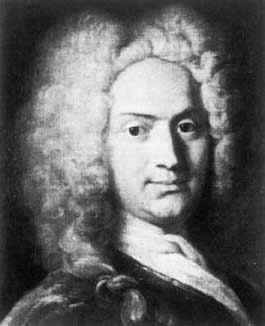
\includegraphics[width=0.8\linewidth,height=\textheight,keepaspectratio]{figures/NBernoulli.jpeg}

\begin{center}\rule{0.5\linewidth}{0.5pt}\end{center}

\subsection{St.~Petersburg Paradox:
History}\label{st.-petersburg-paradox-history-1}

1713: Montmort replies

\begin{quote}
\emph{``It's really easy to calculate the value, just use the EV
calculation techniques that your uncle invented\ldots{}''} --- Pierre
Montmort in 1713 (paraphrasing)
\end{quote}

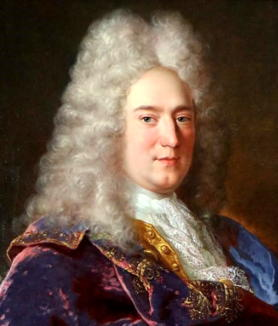
\includegraphics[width=0.8\linewidth,height=\textheight,keepaspectratio]{figures/Montmort.jpg}

\begin{center}\rule{0.5\linewidth}{0.5pt}\end{center}

\subsection{St.~Petersburg Paradox:
History}\label{st.-petersburg-paradox-history-2}

1713: Bernoulli answers

\begin{quote}
\emph{``Yeah, I know how to solve this. But you should have tried
yourself. The solution doesn't make any sense.''} --- Nicolaus Bernoulli
in 1713 (paraphrasing)
\end{quote}

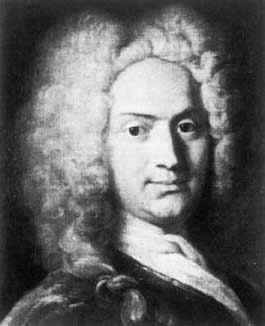
\includegraphics[width=0.8\linewidth,height=\textheight,keepaspectratio]{figures/NBernoulli.jpeg}

\begin{center}\rule{0.5\linewidth}{0.5pt}\end{center}

\subsection{St.~Petersburg Paradox:
History}\label{st.-petersburg-paradox-history-3}

1738: Daniel Bernoulli resolves the paradox

\begin{quote}
\emph{``Just assume \(u'' < 0\).''} --- Daniel Bernoulli in 1738
(paraphrasing)
\end{quote}

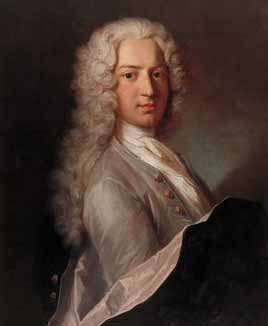
\includegraphics[width=0.8\linewidth,height=\textheight,keepaspectratio]{figures/DBernoulli.jpg}

\begin{center}\rule{0.5\linewidth}{0.5pt}\end{center}

\subsection{Daniel's solution}\label{daniels-solution}

\begin{itemize}
\tightlist
\item
  Assuming that the utility function is concave in money, we can resolve
  the paradox.
\item
  E.g., assume that \(u(z) = \ln(z)\): \[\small
      \sum_{k=1}^{\infty}\left(\frac{1}{2}\right)^k ln(2^{k-1}) = \sum_{k=1}^{\infty}\left(\frac{1}{2}\right)^k (k-1)ln(2) = ln(2)\sum_{k=1}^{\infty}\frac{k-1}{2^k}.
  \]
\item
  Focus on the geometrical series: \[\small
    \sum_{k=1}^{\infty}\frac{k-1}{2^k} = \sum_{k=1}^{\infty}\frac{k}{2^k} - \sum_{k=1}^{\infty}\frac{1}{2^k}.
  \]
\end{itemize}

\begin{center}\rule{0.5\linewidth}{0.5pt}\end{center}

\subsection{Daniel's solution}\label{daniels-solution-1}

\begin{itemize}
\tightlist
\item
  Focus on the geometrical series: \[\small
    \sum_{k=1}^{\infty}\frac{k-1}{2^k} = \sum_{k=1}^{\infty}\frac{k}{2^k} - \sum_{k=1}^{\infty}\frac{1}{2^k} = a - b
  \]
\item
  The term \(b\) is: \[\small
    b = \sum_{k=1}^{\infty}\frac{1}{2^k} = \frac{1}{2}\sum_{k=1}^{\infty}\frac{1}{2^{k-1}} = \frac{1}{2}\left(1 + \frac{1}{2} + \frac{1}{4} + \ldots \right) \\
    = \frac{1}{2}\left(1 + b\right) \Rightarrow b = \frac{1}{2}(1+b) \Rightarrow b = 1
  \]
\end{itemize}

\begin{center}\rule{0.5\linewidth}{0.5pt}\end{center}

\subsection{Daniel's solution}\label{daniels-solution-2}

\begin{itemize}
\tightlist
\item
  Focus on the geometrical series: \[\small
    \sum_{k=1}^{\infty}\frac{k-1}{2^k} = \sum_{k=1}^{\infty}\frac{k}{2^k} - \sum_{k=1}^{\infty}\frac{1}{2^k} = a - b
  \]
\item
  The term \(a\) is: \[\small
    a = \sum_{k=1}^{\infty}\frac{k}{2^k} = \frac{1}{2}\sum_{k=1}^{\infty}\frac{k}{2^{k-1}} = 
    \frac{1}{2}\left(1 + 2\times \frac{1}{2} + 3 \times \frac{1}{4} + \ldots \right) \\
    = \frac{1}{2}\left(1 + \frac{1}{2} + 2\times\frac{1}{4} + 3\times \frac{1}{8} + \ldots + \frac{1}{2} + \frac{1}{4} + \frac{1}{8} + \ldots\right) 
  \]
\end{itemize}

\begin{center}\rule{0.5\linewidth}{0.5pt}\end{center}

\subsection{Daniel's solution}\label{daniels-solution-3}

\begin{itemize}
\tightlist
\item
  Focus on the geometrical series: \[\small
    \sum_{k=1}^{\infty}\frac{k-1}{2^k} = \sum_{k=1}^{\infty}\frac{k}{2^k} - \sum_{k=1}^{\infty}\frac{1}{2^k} = a - b
  \]
\item
  The term \(a\) is: \[\small
    a
    = \frac{1}{2}\left(1 + a + b\right) \Rightarrow a = \frac{1}{2}(2 + a) \Rightarrow a = 2.
  \]
\item
  So the overall lottery value becomes: \[\small
  \ln(2)\times(a - b) = \ln(2).
  \]
\end{itemize}

\begin{center}\rule{0.5\linewidth}{0.5pt}\end{center}

\subsection{Utility Over Money}\label{utility-over-money}

\begin{itemize}
\tightlist
\item
  Since the St.~Petersburg paradox, conventional wisdom that utility is
  concave in money.
\item
  This completes classical theory, which is: \[
  \text{EU / SEU} + \text{concave utility in money.}
  \]
\item
  In the classical theory, agents are \emph{risk-averse} because of the
  way their utility function is shaped.
\end{itemize}

\begin{center}\rule{0.5\linewidth}{0.5pt}\end{center}

\subsection{Empirical Challenges}\label{empirical-challenges}

\begin{itemize}
\tightlist
\item
  Daniel Kahneman~\&~Amos Tversky made a career out of empirically
  testing predictions of the classical theory.
\item
  Kahneman later won a nobel prize for this work.
\item
  Tversky would have won it as well, but he passed away prematurely.
\end{itemize}

\begin{center}\rule{0.5\linewidth}{0.5pt}\end{center}

\subsubsection{Example~}\label{example}

\begin{itemize}
\tightlist
\item
  K\&T provide participants with choices:
\end{itemize}

\textbf{Q1.} Choose between:

\begin{enumerate}
\def\labelenumi{(\Alph{enumi})}
\tightlist
\item
  \(\tiny(0.33, 2500;\,0.66, 2400;\,0.01,0)\)
\item
  2400 for sure.
\end{enumerate}

\textbf{Q2.} Choose between: ~

\begin{enumerate}
\def\labelenumi{(\Alph{enumi})}
\setcounter{enumi}{2}
\tightlist
\item
  \(\tiny(0.33,2500;\,0.67,0)\)
\item
  \(\tiny(0.34,2400;\,0.66,0)\)
\end{enumerate}

\begin{quote}
82\,\% prefer B over A and 83\,\% prefer C over D.
\end{quote}

\begin{center}\rule{0.5\linewidth}{0.5pt}\end{center}

\subsubsection{Example}\label{example-1}

\textbf{Q1.} Choose between:

\begin{enumerate}
\def\labelenumi{(\Alph{enumi})}
\tightlist
\item
  \(\tiny(0.33, 2500;\,0.66, 2400;\,0.01,0)\)
\item
  2400 for sure.
\end{enumerate}

\textbf{Q2.} Choose between: ~

\begin{enumerate}
\def\labelenumi{(\Alph{enumi})}
\setcounter{enumi}{2}
\tightlist
\item
  \(\tiny(0.33,2500;\,0.67,0)\)
\item
  \(\tiny(0.34,2400;\,0.66,0)\)
\end{enumerate}

\begin{itemize}
\item
  \(B\succ A\) implies: \[
  \small
  u(24k) > 0.33 u(25k) + 0.66 u(24k) \Rightarrow 0.34u(24k) > 0.33u(25k). 
  \]
\item
  \(C\succ D\) implies: \(\small 0.33 u(25k) > 0.34 u(24k),\) a
  contradiction.
\end{itemize}

\begin{center}\rule{0.5\linewidth}{0.5pt}\end{center}

\subsubsection{Example 2}\label{example-2}

\textbf{Q1.} Choose between:

\begin{enumerate}
\def\labelenumi{(\Alph{enumi})}
\tightlist
\item
  3 week England, France, Italy tour w/ 50\%
\item
  1 week England tour
\end{enumerate}

\textbf{Q2.} Choose between: ~

\begin{enumerate}
\def\labelenumi{(\Alph{enumi})}
\setcounter{enumi}{2}
\tightlist
\item
  3 week England, France, Italy tour w/ 5\%.
\item
  1 week England tour w/ 10\%.
\end{enumerate}

\begin{quote}
77\% prefer B over A and 67\% prefer C over D.
\end{quote}

\begin{itemize}
\tightlist
\item
  Q2 is just a compounded version of Q1, so independence predicts that
  \(D\succ C\) if \(B\succ A\).
\end{itemize}

\begin{center}\rule{0.5\linewidth}{0.5pt}\end{center}

\subsubsection{People prefer safe over
risky}\label{people-prefer-safe-over-risky}

\textbf{Q1.} Choose between:

\begin{enumerate}
\def\labelenumi{(\Alph{enumi})}
\tightlist
\item
  \(\scriptstyle (0.33, 2500;\,0.66, 2400;\,0.01,0)\)
\item
  \textbf{2400 for sure.}
\end{enumerate}

\textbf{Q2.} Choose between: ~

\begin{enumerate}
\def\labelenumi{(\Alph{enumi})}
\setcounter{enumi}{2}
\tightlist
\item
  \(\boldsymbol{(0.33,2500;\,0.67,0)}\)
\item
  \((0.34,2400;\,0.66,0)\)
\end{enumerate}

\textbf{Q1.} Choose between:

\begin{enumerate}
\def\labelenumi{(\Alph{enumi})}
\tightlist
\item
  3 week England, France, Italy tour w/ 50\%
\item
  \textbf{1 week England tour}.
\end{enumerate}

\textbf{Q2.} Choose between: ~

\begin{enumerate}
\def\labelenumi{(\Alph{enumi})}
\setcounter{enumi}{2}
\tightlist
\item
  \textbf{3 week England, France, Italy tour w/ 5\%.}
\item
  1 week England tour w/ 10\%.
\end{enumerate}

\begin{center}\rule{0.5\linewidth}{0.5pt}\end{center}

\subsubsection{Small probabilities}\label{small-probabilities}

The certainty effect does not hold when probabilities are small.

Choose between:

\begin{enumerate}
\def\labelenumi{(\Alph{enumi})}
\tightlist
\item
  0.1\% chance of 5000.
\item
  5 for sure.
\end{enumerate}

\begin{quote}
72\% prefer the uncertain option (A)
\end{quote}

\begin{itemize}
\tightlist
\item
  In contradiction with \(EU + \text{concave utility}.\)
\end{itemize}

\begin{center}\rule{0.5\linewidth}{0.5pt}\end{center}

\subsubsection{Sensitivity to absolute
differences}\label{sensitivity-to-absolute-differences}

\textbf{Q1.} Choose between:

\begin{enumerate}
\def\labelenumi{(\Alph{enumi})}
\tightlist
\item
  \((0.001, 6000; 0.999, 0)\)
\item
  \((0.002, 3000; 0.998, 0)\)
\end{enumerate}

\textbf{Q2.} Choose between:

\begin{enumerate}
\def\labelenumi{(\Alph{enumi})}
\setcounter{enumi}{2}
\tightlist
\item
  \((0.45, 6000; 0.55, 0)\)
\item
  \((0.9, 3000; 0.1, 0)\)
\end{enumerate}

\begin{quote}
73\% choose A over B and 86\% choose D over C.
\end{quote}

\begin{itemize}
\item
  \(A\succ B\) implies
  \(0.001 u(6k) > 0.002 u(3k) \Rightarrow \frac{u(6k)}{u(3k)} > 2.\)
\item
  But then, \(0.45 u(6k)  > 0.9 u(3k) \Rightarrow C \succ D.\)
\end{itemize}

\begin{center}\rule{0.5\linewidth}{0.5pt}\end{center}

\subsection{Generalizing from
examples}\label{generalizing-from-examples}

\begin{itemize}
\tightlist
\item
  These examples all come from Kahneman and Tversky (ECTA, 1979).
\item
  Kahneman and Tversky develop an alternative theory to accommodate
  findings that, relative to EU:

  \begin{itemize}
  \tightlist
  \item
    Individuals prefer certain prospects to uncertain prospects,
  \item
    they overweight small probabilities,
  \item
    are more sensitive to large than small absolute differences in
    probability.
  \end{itemize}
\item
\end{itemize}

\begin{center}\rule{0.5\linewidth}{0.5pt}\end{center}

\subsection{Probability weighting}\label{probability-weighting}

\begin{itemize}
\tightlist
\item
  K\&T propose a theory of \textbf{probability weighting.}
\item
  Remember that EU weighting is linear: \(EU = \sum_z p(z)u(z),\) where
  \(p(z)\) is probability of \(z.\)
\item
  K\&T propose: \(\sum_z\pi(p(z))u(z),\) where \(\pi(p)\) is
  \emph{nonlinear.}
\end{itemize}

\begin{center}\rule{0.5\linewidth}{0.5pt}\end{center}

\subsection{Probability weighting}\label{probability-weighting-1}

\begin{itemize}
\tightlist
\item
  K\&T propose: \(\sum_z\pi(p(z))u(z),\) where \(\pi(p)\) is nonlinear.
\end{itemize}

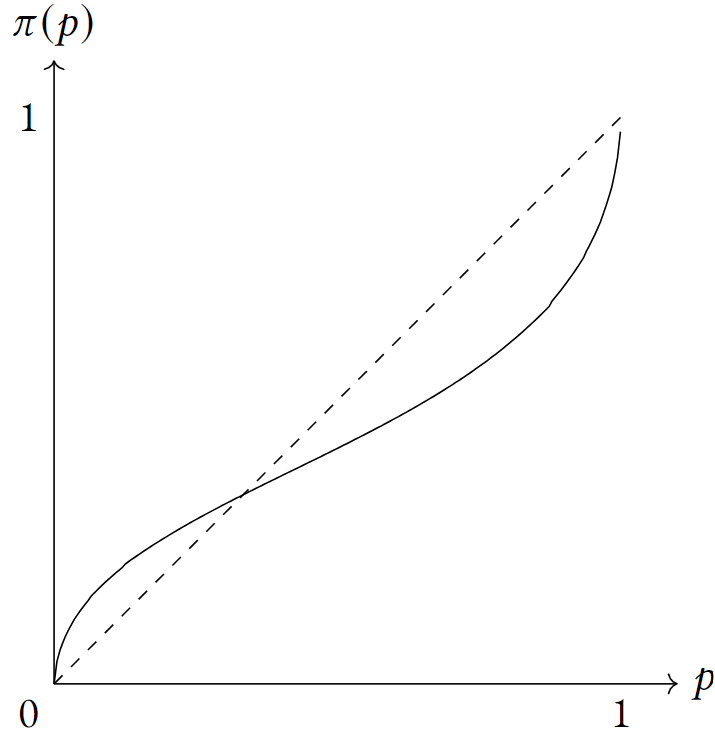
\includegraphics[width=0.85\linewidth,height=\textheight,keepaspectratio]{figures/WeightingFunction.png}

\begin{itemize}
\tightlist
\item
  \emph{Regularity:} \(\scriptstyle \pi(0) = 0,\,\pi(1) = 1\)
\item
  \emph{Overweighting of small \(p\):} \(\pi(p)>p\) if \(p < \hat{p}\)
\item
  \emph{Subcertainty:} \(\scriptstyle \pi(p) + \pi(1-p) < 1\)
\item
  \emph{Subproportionality:}
  \(\scriptstyle\frac{\pi(pq)}{\pi(p)} \leq \frac{\pi(pqr)}{\pi(pr)}\)
  for \(\scriptstyle p,q,r\in(0,1)\)
\end{itemize}

\begin{center}\rule{0.5\linewidth}{0.5pt}\end{center}

\subsection{}\label{section}

\subsubsection{Probability weigthing:
Implications}\label{probability-weigthing-implications}

\begin{itemize}
\tightlist
\item
  Probability weighting fits the data better than EU/SEU linear
  weighting.
\item
  Different from classical theory, probability weighting can explain
  risk attitudes through probability perceptions:

  \begin{itemize}
  \tightlist
  \item
    Overweighting of small prob: Risk-seeking for small \(p\).
  \item
    Underweigthing of large prob: Risk-aversion for large \(p\).
  \end{itemize}
\end{itemize}

\begin{center}\rule{0.5\linewidth}{0.5pt}\end{center}

\subsection{}\label{section-1}

\subsubsection{Probability weigthing:
Implications}\label{probability-weigthing-implications-1}

\begin{itemize}
\tightlist
\item
  Probability weighting fits the data better than EU/SEU linear
  weighting.
\item
  Probability weigthing is {descriptive}, not {prescriptive}.

  \begin{itemize}
  \tightlist
  \item
    Different from classical theory, which derives behavior from
    normatively \emph{desirable} axioms.
  \end{itemize}
\end{itemize}

\begin{itemize}
\tightlist
\item
  This raises the question of whether probability weighting is
  deliberate or a mistake.
\item
  Some modern debate about this (next).
\end{itemize}

\begin{center}\rule{0.5\linewidth}{0.5pt}\end{center}

\subsection{Measuring probability
weighting}\label{measuring-probability-weighting}

\begin{itemize}
\tightlist
\item
  Standard method of eliciting \textbf{risk attitudes} in experimental
  econ: Use a multiple price list (MPL) to measure a \textbf{certainty
  equivalent.}
\end{itemize}

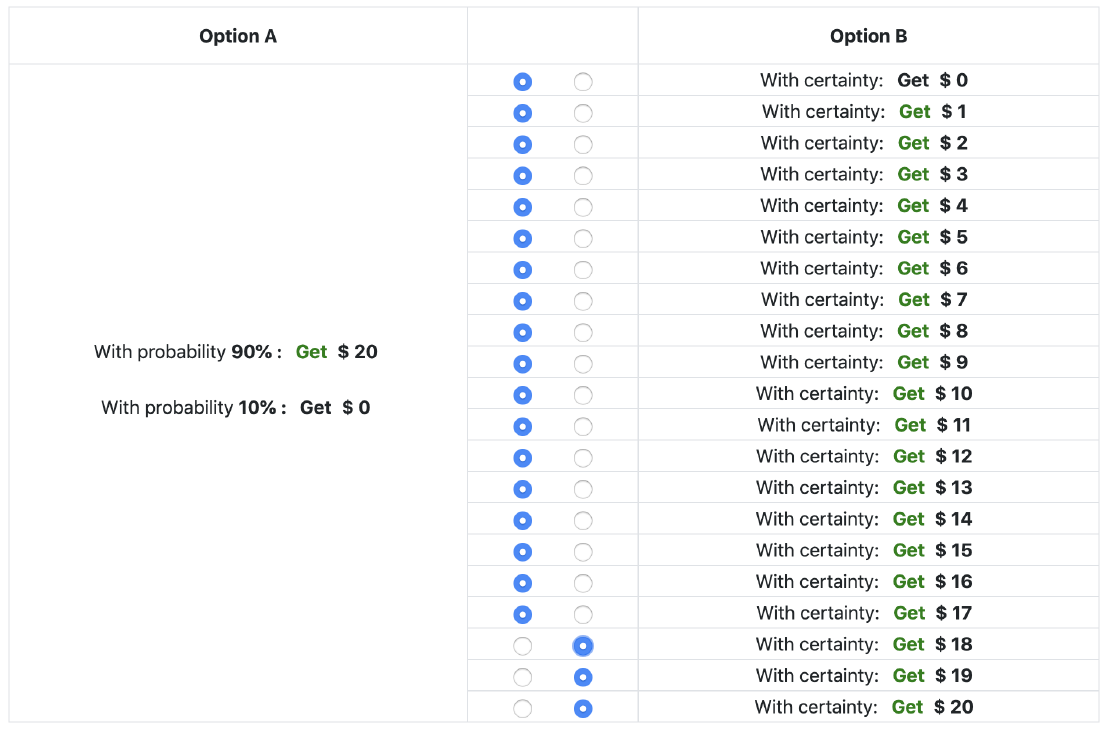
\includegraphics[width=0.45\linewidth,height=\textheight,keepaspectratio]{figures/CognitiveUncertaintyMPL.png}

\begin{itemize}
\tightlist
\item
  Here, CE of lottery is between \$17 and \$18.
\end{itemize}

\begin{center}\rule{0.5\linewidth}{0.5pt}\end{center}

\subsection{Measuring probability
weighting}\label{measuring-probability-weighting-1}

\begin{itemize}
\tightlist
\item
  With \emph{binary} lotteries, which pay X€ with \(p\) and nothing with
  \(1-p\), we can identify risk attitudes from CE:

  \begin{itemize}
  \tightlist
  \item
    Risk neutral if \(CE = p X.\)
  \item
    Risk averse if \(CE < p X.\)
  \item
    Risk seeking if \(CE > p X.\)
  \end{itemize}
\item
  Often, we use \emph{normalized} CEs, which are
  \(\widetilde{CE} = \frac{CE}{X}.\)

  \begin{itemize}
  \tightlist
  \item
    Risk neutral if \(\widetilde{CE} = p.\)
  \item
    Risk averse if \(\widetilde{CE} < p.\)
  \item
    Risk seeking if \(\widetilde{CE} > p.\)
  \end{itemize}
\end{itemize}

\begin{center}\rule{0.5\linewidth}{0.5pt}\end{center}

\subsection{Measuring probability
weighting}\label{measuring-probability-weighting-2}

\begin{itemize}
\tightlist
\item
  Assuming utility is \emph{linear} in money, we can use CEs to back out
  \(\pi(p)\): \[
  \pi(1)u(CE) = \pi(p)u(X) \Rightarrow \pi(1)(a + b\cdot CE) = \pi(p)(a + b\cdot X) \\
  \text{assume }a=0 \text{ w/o loss and }\pi(1) = 1\\ 
  \Rightarrow 
  \pi(p) = \frac{CE}{X} \Rightarrow \pi(p)  = \widetilde{CE}.
  \]
\item
  Thus, assuming linear utilities allows to back out nonlinear
  \(\pi(p)\).
\end{itemize}

\begin{center}\rule{0.5\linewidth}{0.5pt}\end{center}

\subsubsection{Linking probability weighting to cognitive
mistakes}\label{linking-probability-weighting-to-cognitive-mistakes}

\begin{itemize}
\tightlist
\item
  Enke and Graeber (QJE, 2023) link PW to individual confidence about
  decisions.
\item
  They elicit CE and ask:
\end{itemize}

\begin{quote}
\emph{Your decision on the previous screen indicates that you value this
lottery as much as receiving \$x with certainty. How certain are you
that you actually value this lottery somewhere between getting
\$(x−0.50) and \$(x+0.50)?}
\end{quote}

\begin{center}\rule{0.5\linewidth}{0.5pt}\end{center}

\subsubsection{Enke and Graeber (QJE, 2023): People who are more
uncertain about their choices weight probabilities more
strongly}\label{enke-and-graeber-qje-2023-people-who-are-more-uncertain-about-their-choices-weight-probabilities-more-strongly}

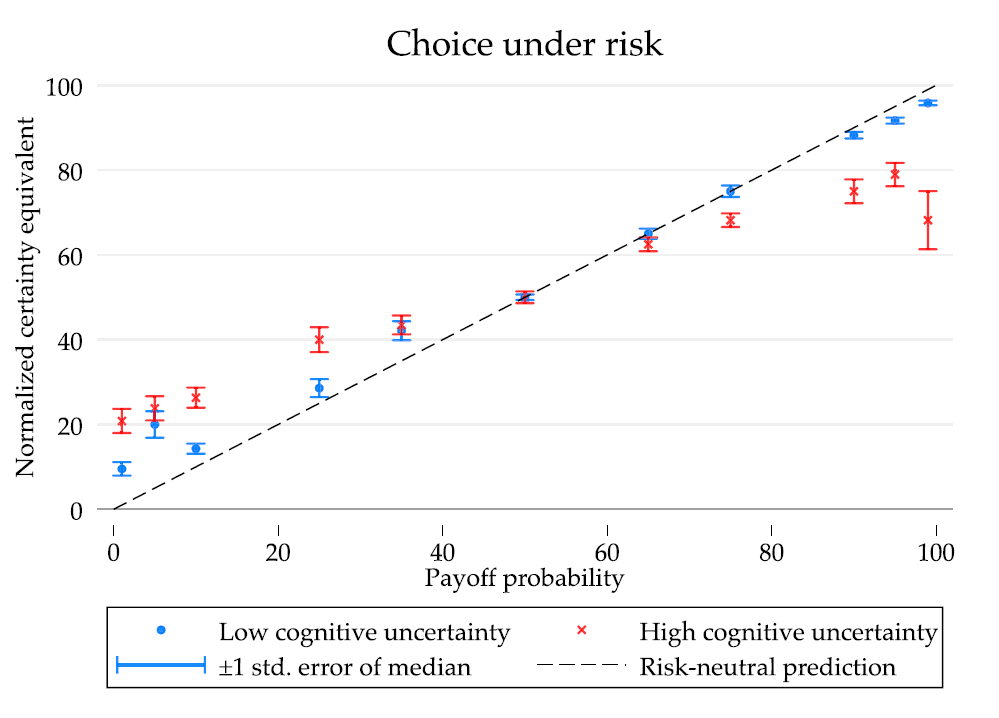
\includegraphics[width=0.7\linewidth,height=\textheight,keepaspectratio]{figures/CognitiveUncertaintyRisk.png}

\begin{center}\rule{0.5\linewidth}{0.5pt}\end{center}

\subsubsection{Complexity as a reason for probability
weighting?}\label{complexity-as-a-reason-for-probability-weighting}

\begin{itemize}
\tightlist
\item
  The previous evidence suggests the following interpretation:

  \begin{itemize}
  \tightlist
  \item
    Individuals who find calculating lottery payoffs easy are almost
    risk neutral.
  \item
    Individuals who find this difficult act \emph{as if} they weight
    probabilities.
  \end{itemize}
\item
  But the evidence is correlational, not causal.
\item
  Oprea (AER, 2024) investigates the \emph{causal link} between task
  complexity and probability weighting.
\end{itemize}

\begin{center}\rule{0.5\linewidth}{0.5pt}\end{center}

\subsubsection{Mirror experiment in Oprea (AER,
2024)}\label{mirror-experiment-in-oprea-aer-2024}

\begin{itemize}
\tightlist
\item
  Main idea: Risky decisions are difficult, because people need to
  calculate an expected payoff, etc.
\item
  For example, suppose that, when seeing a lottery \((10, p; 5, 1-p)\),
  people approximate \(p\) with 50\% to simplify calculations.
\item
  So instead of calculating \(EU = p u(10)+ (1-p)u(5),\) they
  approximate \(EU\approx 0.5 u(10) + 0.5 u(5).\)
\item
  This would yield the effect of \emph{overweighting small
  probabilities} and \emph{underweighting large ones}.
\end{itemize}

\begin{center}\rule{0.5\linewidth}{0.5pt}\end{center}

\subsubsection{Mirror experiment in Oprea (AER,
2024)}\label{mirror-experiment-in-oprea-aer-2024-1}

\begin{itemize}
\tightlist
\item
  Oprea creates compares risky MPL decisions to nonrisky ``mirror''
  decisions.
\end{itemize}

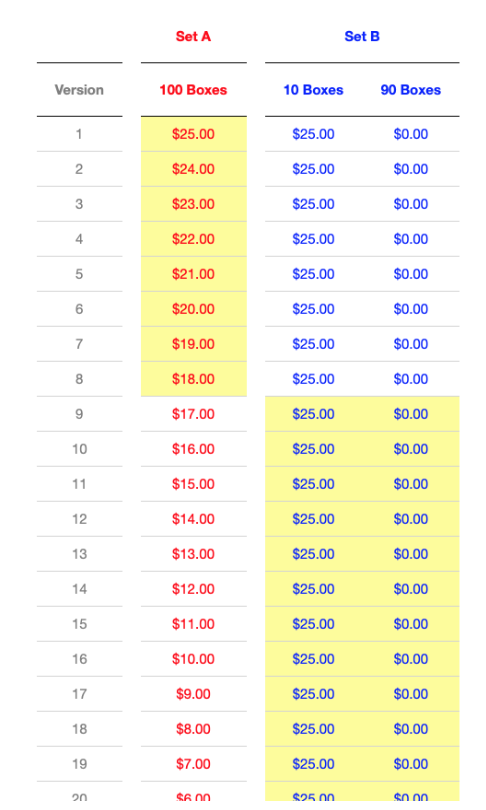
\includegraphics[width=0.85\linewidth,height=\textheight,keepaspectratio]{figures/SimplicityEquivalentsMPL.png}

\begin{itemize}
\tightlist
\item
  When opening one random box from Set B, this is a risky choice.
\item
  When taking the EV over all Set B boxes, this is a complex, nonrisky
  ``mirror'' choice.
\item
  Oprea compares \emph{risky} to \emph{mirror}.
\end{itemize}

\begin{center}\rule{0.5\linewidth}{0.5pt}\end{center}

\subsubsection{Oprea (AER, 2024): Risky decisions = Mirror
decisions}\label{oprea-aer-2024-risky-decisions-mirror-decisions}

\begin{itemize}
\tightlist
\item
  Estimated ``probability weight'' is no different under {risk (white)}
  and {mirror (gray)}.
\end{itemize}

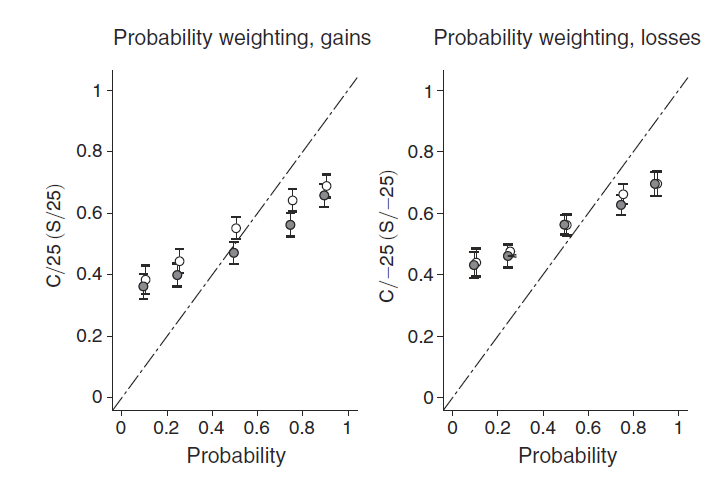
\includegraphics[width=0.55\linewidth,height=\textheight,keepaspectratio]{figures/SimplicitlyEquivalents.png}

\begin{center}\rule{0.5\linewidth}{0.5pt}\end{center}

\subsubsection{Are risk attitudes simply
mistakes?}\label{are-risk-attitudes-simply-mistakes}

\begin{itemize}
\tightlist
\item
  In mirror task, not switching where \(CE = EV\) is clearly a mistake.
\item
  Since risky decisions look like mirror decisions, tempting to argue
  that any form of risk attitude is due to the same type of calculation
  mistake.
\item
  But critique of Oprea (2024) quickly followed:

  \begin{itemize}
  \tightlist
  \item
    The design is \emph{weird,} mirror task can seem like a trick
    question.
  \item
    Participants may mistakenly treat mirror decisions as choices under
    risk\ldots{}
  \end{itemize}
\end{itemize}

\begin{center}\rule{0.5\linewidth}{0.5pt}\end{center}

\subsection{}\label{section-2}

\subsubsection{Misunderstandings in Oprea (AER,
2024)}\label{misunderstandings-in-oprea-aer-2024}

\begin{itemize}
\tightlist
\item
  Oprea asked participants comprehension questions about the
  instructions.
\item
  Banki et al (WP, 2025) show that participants who did not make
  comprehension mistakes show differences between lotteries and mirrors.
\end{itemize}

\begin{center}\rule{0.5\linewidth}{0.5pt}\end{center}

\subsection{}\label{section-3}

\subsubsection{Misunderstandings in Oprea (AER,
2024)}\label{misunderstandings-in-oprea-aer-2024-1}

\begin{itemize}
\tightlist
\item
  Banki et al (WP, 2025) show that participants who did not make
  comprehension mistakes show differences between lotteries and mirrors.
\end{itemize}

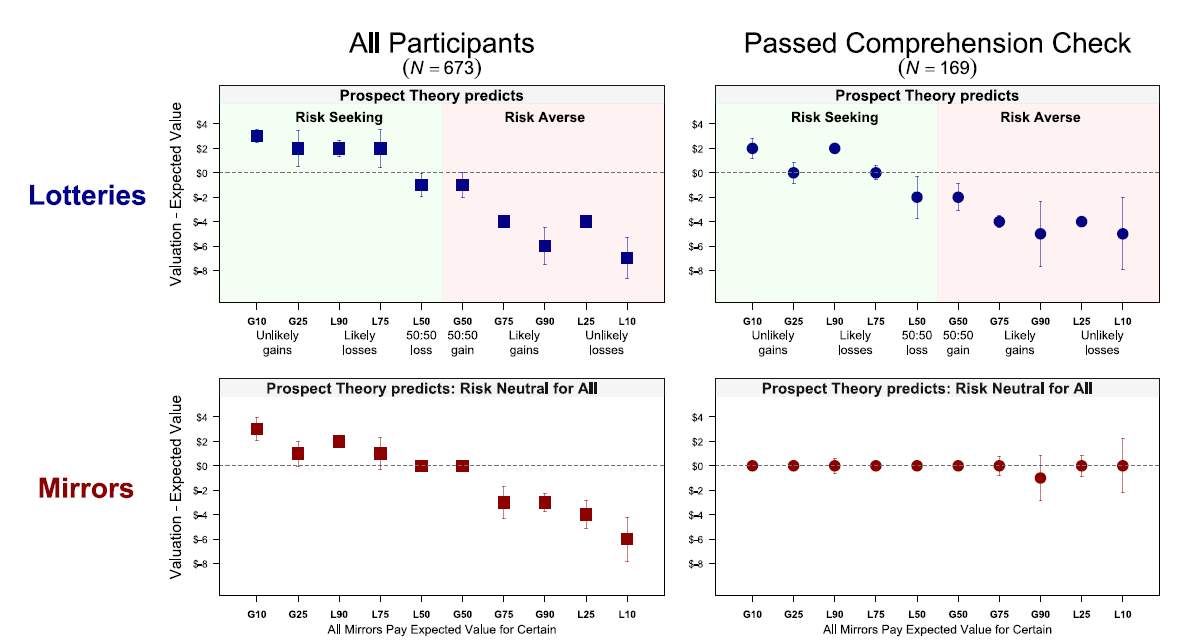
\includegraphics[width=0.7\linewidth,height=\textheight,keepaspectratio]{figures/SimplicityEquivalentsComment.png}

\begin{center}\rule{0.5\linewidth}{0.5pt}\end{center}

\subsection{}\label{section-4}

\subsubsection{Misunderstandings in Oprea (AER,
2024)}\label{misunderstandings-in-oprea-aer-2024-2}

\begin{itemize}
\tightlist
\item
  Banki et al (WP, 2025) show that participants who did not make
  comprehension mistakes show differences between lotteries and mirrors.
\end{itemize}

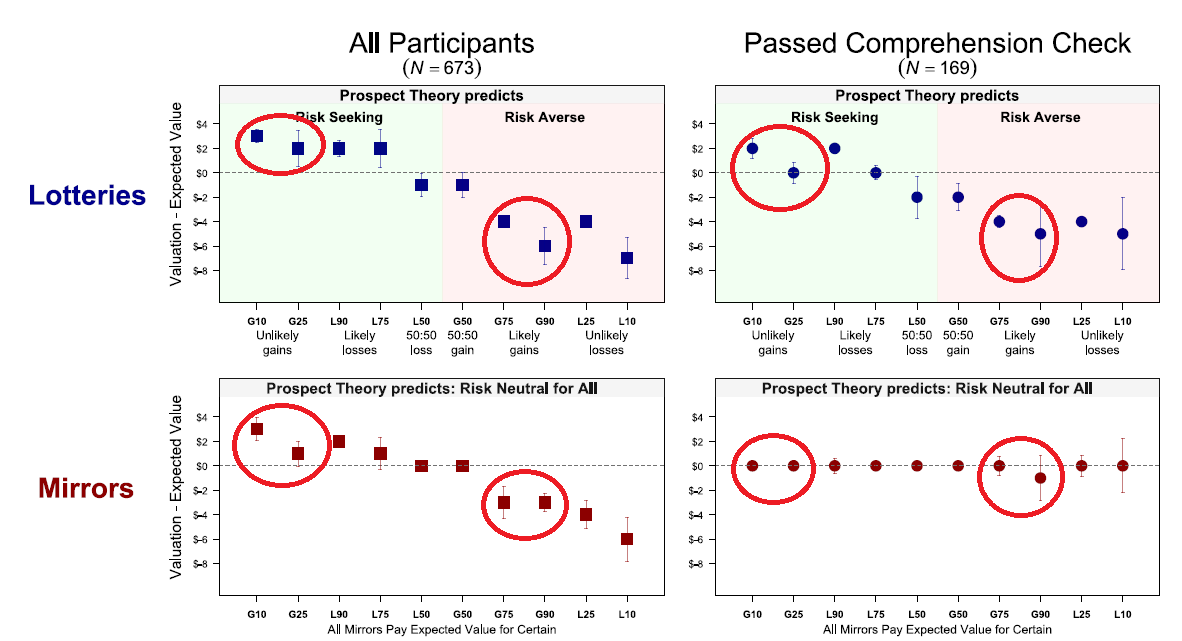
\includegraphics[width=0.7\linewidth,height=\textheight,keepaspectratio]{figures/SimplicityEquivalentsCommentRed.png}

\begin{center}\rule{0.5\linewidth}{0.5pt}\end{center}

\subsubsection{Wu (WP, 2025): Mirrors are different from
lotteries}\label{wu-wp-2025-mirrors-are-different-from-lotteries}

\begin{itemize}
\tightlist
\item
  In a follow-up, Wu (WP, 2025) claims to provide clearer instructions
  when comparing mirrors to choice \& finds that choices are different.
\item
  Participants select: \$X for sure or \$100 with \(P.\)
\end{itemize}

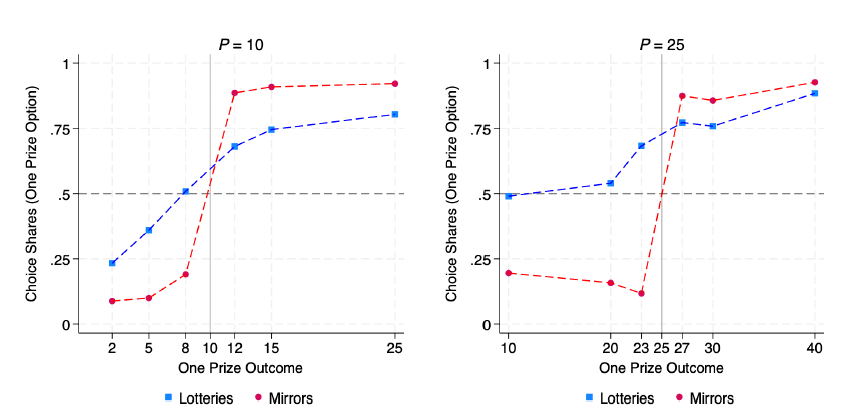
\includegraphics[width=0.6\linewidth,height=\textheight,keepaspectratio]{figures/SimplicityEquivalentsWu.png}

\begin{center}\rule{0.5\linewidth}{0.5pt}\end{center}

\subsection{Takeaways}\label{takeaways}

\begin{itemize}
\tightlist
\item
  Decisions under risk are special.

  \begin{itemize}
  \tightlist
  \item
    Individuals overweight small probabilities and underweight large
    ones.
  \end{itemize}
\item
  This is not \emph{only} driven by calculation complexity.

  \begin{itemize}
  \tightlist
  \item
    But complexity is part of the story.
  \end{itemize}
\item
  The other part seems to reflect genuine preferences or risk attitudes.
\end{itemize}

{\textbf{Is probability weighting a mistake?}}

\begin{itemize}
\tightlist
\item
  If you find the EU axioms desirable, then yes.
\end{itemize}

\begin{center}\rule{0.5\linewidth}{0.5pt}\end{center}

\subsection{``Fixing'' a ``flaw'' in PW}\label{fixing-a-flaw-in-pw}

\begin{itemize}
\tightlist
\item
  While descriptively valid, PW can make strange predictions.
\item
  Consider \[
  L_A = (x, 0.1;x, 0.1;x, 0.1;x, 0.1; 0, 0.6),\, 
  L_B = (x, 0.4; 0, 0.6).
  \]
\item
  Both lotteries generate the same outcomes, but PW may predict strict
  preference for \(L_A\); if \(\pi(0.1) > 0.1\) and
  \(\pi(0.4)\approx 0.4\), then \[
  4\pi(0.1)u(x) + \pi(0.6)u(0) > \pi(0.4)u(x) + \pi(0.6)u(0).
  \]
\end{itemize}

\begin{center}\rule{0.5\linewidth}{0.5pt}\end{center}

\subsection{}\label{section-5}

\subsubsection{``Fixing'' a ``flaw'' in PW}\label{fixing-a-flaw-in-pw-1}

\begin{itemize}
\tightlist
\item
  As an implication, PW may violate \textbf{dominance.}
\end{itemize}

\textbf{Dominance.} If one lottery always provides an outcome at least
as good as another lottery in every state of the world, and is strictly
better in at least one state, then this lottery should be preferred.

\begin{center}\rule{0.5\linewidth}{0.5pt}\end{center}

\subsection{}\label{section-6}

\subsubsection{``Fixing'' a ``flaw'' in PW}\label{fixing-a-flaw-in-pw-2}

\textbf{Dominance.} If one lottery always provides an outcome at least
as good as another lottery in every state of the world, and is strictly
better in at least one state, then this lottery should be preferred.

E.g., consider \(L_A = (x, p; 0, 1-p)\) and
\(L_B = (x, p/2; x - \varepsilon, p/2; 0, 1-p),\) where
\(\varepsilon > 0\). Clearly, \(L_A\) \emph{dominates} \(L_B\).

\begin{center}\rule{0.5\linewidth}{0.5pt}\end{center}

\subsection{}\label{section-7}

\subsubsection{``Fixing'' a ``flaw'' in PW}\label{fixing-a-flaw-in-pw-3}

Because \(\pi(p)\) is flat for intermediate values of \(p,\) dominated
lotteries may be preferred.

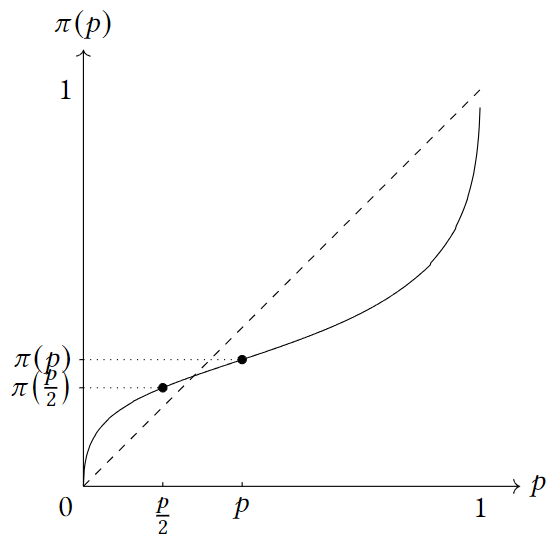
\includegraphics[width=0.5\linewidth,height=\textheight,keepaspectratio]{figures/Dominance.png}

\begin{center}\rule{0.5\linewidth}{0.5pt}\end{center}

\subsection{}\label{section-8}

\subsubsection{Fixing with
rank-dependency}\label{fixing-with-rank-dependency}

\begin{itemize}
\tightlist
\item
  Tversky and Kahneman (JRU, 1992) propose \textbf{rank-dependent} (or
  \emph{cumulative}) probability weights to avoid dominance violations.
\item
  Consider a lottery \(L = (X, p; Y, q; Z, 1-p-q),\) where \(X>Y>Z\) and
  an alternative lottery \(L' = (Z,1) + (Y-Z, p + q) + (X-Y,p).\)
\item
  An EU agent is indifferent between \(L\) and \(L':\) \[
  EU(L) = p u(X) + q u(Y) + (1-p-q)u(Z)  \\
  = u(Z) + (p+q)[u(Y) - u(Z)] + p[u(X) - u(Z)] = EU(L').
  \]
\end{itemize}

\begin{center}\rule{0.5\linewidth}{0.5pt}\end{center}

\subsection{}\label{section-9}

\subsubsection{Fixing with
rank-dependency}\label{fixing-with-rank-dependency-1}

\begin{itemize}
\tightlist
\item
  An EU agent is indifferent between \(L\) and \(L':\) \[
  EU(L) = p u(X) + q u(Y) + (1-p-q)u(Z)  \\
  = u(Z) + (p+q)[u(Y) - u(Z)] + p[u(X) - u(Z)] = EU(L').
  \]
\item
  With rank dependent weights, we assume that the agent always mentally
  transforms \(L\) to \(L'\) before calculating probability weights: \[
  EU_\pi(L) = \boldsymbol{\pi(1)}u(Z) + \boldsymbol{[\pi(p) + \pi(q)]}[u(Y) - u(Z)] +
  \\ \boldsymbol{\pi(p)}[u(X) - u(Z)].
  \]
\end{itemize}

\begin{center}\rule{0.5\linewidth}{0.5pt}\end{center}

\subsection{}\label{section-10}

\subsubsection{Fixing with
rank-dependency}\label{fixing-with-rank-dependency-2}

\begin{itemize}
\tightlist
\item
  With rank dependent weights, rewrite lotteries in the \(L'\) way.
  Then, add weights: \[
  EU_\pi(L) = \boldsymbol{\pi(1)}u(Z) + \boldsymbol{[\pi(p) + \pi(q)]}[u(Y) - u(Z)] +
  \\ \boldsymbol{\pi(p)}[u(X) - u(Z)].
  \]
\item
  More commonly this is (equivalently) written as \[
  EU_\pi(L) = \pi(p)u(X) + [\pi(p+q) - \pi(p)]u(Y) + 
  \\ [\pi(1) - \pi(p + q)]u(Z).
  \]
\end{itemize}

\begin{center}\rule{0.5\linewidth}{0.5pt}\end{center}

\subsection{}\label{section-11}

\subsubsection{Rank-dependent weights fix the dominance
problem}\label{rank-dependent-weights-fix-the-dominance-problem}

\begin{itemize}
\tightlist
\item
  We considered: \[
  \scriptsize
  L_A = (x, p; 0, 1-p),\, L_B = (x, p/2; x - \varepsilon, p/2; 0, 1-p), \varepsilon > 0
  \]
\item
  With rank-dependence: \[
  \scriptsize
  EU_\pi(L_A) = \pi(p)u(x) + [\pi(1)-\pi(p)]u(0), \\ 
  \scriptsize
  EU_\pi(L_B) = \pi(p/2)u(x) + [\pi(p) - \pi(p/2)]u(x - \varepsilon) + [\pi(1) - \pi(p)]u(0)
  \]
\item
  Therefore,
  \(\scriptsize EU_\pi(L_A) > EU_\pi(L_B) \Rightarrow u(x) > u(x-\varepsilon).\)
\end{itemize}

\begin{center}\rule{0.5\linewidth}{0.5pt}\end{center}

\subsubsection{Rank-dependent weights fix the dominance
problem}\label{rank-dependent-weights-fix-the-dominance-problem-1}

\begin{itemize}
\tightlist
\item
  Common assertion is that rank-dependent weighting ``refines'' the
  original version.
\item
  Rank-dependent weights are the only way to combine (i) nonlinear
  probability weighting and (ii) nonviolation of dominance.
\item
  But note that there is no empirical motivation for rank-dependence.
\item
  We will explore the empirical validity next.
\end{itemize}

\begin{center}\rule{0.5\linewidth}{0.5pt}\end{center}

\subsubsection{Testing for rank
dependency}\label{testing-for-rank-dependency}

\begin{itemize}
\tightlist
\item
  Main idea of a test: With rank-dependence, the probability weight
  associated with a payoff \(X\) depends on the rank of \(X\) relative
  to other possible payoffs. E.g., \[
  \bar{L} = (\bar{X}, p; Y, q; Z, 1-p-q),\, \\ 
  \underline{L} = (\underline{X}, p; Y, q; Z, 1-p-q), \\
  \bar{X} > Y > \underline{X} > Z.
  \]
\end{itemize}

\begin{center}\rule{0.5\linewidth}{0.5pt}\end{center}

\subsection{}\label{section-12}

\begin{itemize}
\tightlist
\item
  Rank-dependent weights predict that \[
  \scriptsize
  EU_\pi(\bar{L}) = \pi(p)u(\bar{X}) + [\pi(p+q) - \pi(p)]u(Y) + [\pi(1) - \pi(p+q)]u(Z), \\
  \scriptsize
  EU_\pi(\underline{L}) = \pi(q)u(Y) + [\pi(p+q) - \pi(p)]u(\underline{X}) + [\pi(1) - \pi(p+q)]u(Z).
  \]
\end{itemize}

\begin{center}\rule{0.5\linewidth}{0.5pt}\end{center}

\subsection{}\label{section-13}

\begin{itemize}
\tightlist
\item
  Rank-dependent weights predict that \[
  \scriptsize
  EU_\pi(\bar{L}) = \boldsymbol{\pi(p)}u(\bar{X}) + \boldsymbol{[\pi(p+q) - \pi(p)]}u(Y) + [\pi(1) - \pi(p+q)]u(Z), \\
  \scriptsize
  EU_\pi(\underline{L}) = \boldsymbol{\pi(q)}u(Y) + \boldsymbol{[\pi(p+q) - \pi(p)]}u(\underline{X}) + [\pi(1) - \pi(p+q)]u(Z).
  \]
\item
  By comparing lotteries such as \(\bar{L}\) and \(\underline{L},\) we
  can test for rank-dependent weights.
\item
  But the problem is that we do not observe \(\pi(p)\). Thus, we need to
  find ways of approximating it.
\end{itemize}

\begin{center}\rule{0.5\linewidth}{0.5pt}\end{center}

\subsection{}\label{section-14}

\subsubsection{Bernheim and Sprenger (ECTA, 2020): Testing for
rank-dependence}\label{bernheim-and-sprenger-ecta-2020-testing-for-rank-dependence}

\begin{itemize}
\tightlist
\item
  Bernheim and Sprenger show that changes in probability weights can be
  approximated by changes in ``equivalent variations''. Participants
  observe lotteries \[
  L = (X, p; Y, q; Z, 1-p-q), \\
  L_e = (X, p; Y + \boldsymbol{m}, q; Z-\boldsymbol{k},1-p-q)
  \]
\item
  Participants observe \(m\) and choose \(k\) so that \(L\sim L_e\).
  I.e., they decide how much of \(Z\) they are willing to give up if
  \(Y\) increases by \(m.\)
\end{itemize}

\begin{center}\rule{0.5\linewidth}{0.5pt}\end{center}

\subsection{}\label{section-15}

\begin{itemize}
\tightlist
\item
  Participants observe \(m\) and choose \(k\) so that \(L\sim L_e\).
  I.e., they decide how much of \(Z\) they are willing to give up if
  \(Y\) increases by \(m.\)
\item
  \textbf{Why:} The equivalent variation \(k\) measures how much I value
  a marginal increase in \(Y\). This valuation depends on the
  probability weight I put on the chance of \(Y\) realizing. Therefore,
  I can learn about the weight by eliciting \(k\).
\item
  \textbf{Idea:} Elicit \(\bar{k}\) and \(\underline{k}\) in lotteries
  \[
  \bar{L}_e = (\bar{X}, p; Y + m, q; Z-\bar{k},1-p-q), \\
  \underline{L}_e = (\underline{X}, p; Y + m, q; Z-\underline{k},1-p-q).
  \]
\end{itemize}

\begin{center}\rule{0.5\linewidth}{0.5pt}\end{center}

\subsection{}\label{section-16}

\subsubsection{Equivalent variations proxy for
weights}\label{equivalent-variations-proxy-for-weights}

\textbf{Proposition.} As \(m\to 0,\) the percentage change in \(k\) when
increasing \(X\) from \(\underline{X} < Y\) to \(\bar{X} > Y\) is
equivalent to the percentage change in the probability weight put on
\(Y\) relative to \(Z.\)

Suppose that the agent values lotteries \(\bar{L}\) and
\(\underline{L}\) as \[
\small
EU(\bar{L}) = \bar{w}_X u(X) + \bar{w}_Y u(Y) + \bar{w}_Z u(Z),\, \\
\small
EU(\underline{L}) = \underline{w}_X u(X) + \underline{w}_Y u(Y) + \underline{w}_Z u(Z).
\]

\begin{center}\rule{0.5\linewidth}{0.5pt}\end{center}

\subsection{}\label{section-17}

\subsubsection{Equivalent variations proxy for
weights}\label{equivalent-variations-proxy-for-weights-1}

\textbf{Proposition.} As \(m\to 0,\) the percentage change in \(k\) when
increasing \(X\) from \(\underline{X} < Y\) to \(\bar{X} > Y\) is
equivalent to the percentage change in the probability weight put on
\(Y\) relative to \(Z.\)

The proposition suggests that: \[
\small \lim_{m\to 0} \ln(\bar{k}) - \ln(\underline{k}) = \ln\left(\frac{\bar{w}_Y}{\bar{w}_z}\right) - \ln\left(\frac{\underline{w}_Y}{\underline{w}_z}\right).
\]

(Proof on board)

\begin{center}\rule{0.5\linewidth}{0.5pt}\end{center}

\subsection{}\label{section-18}

\subsubsection{Equivalent variations allow tests for
rank-dependence}\label{equivalent-variations-allow-tests-for-rank-dependence}

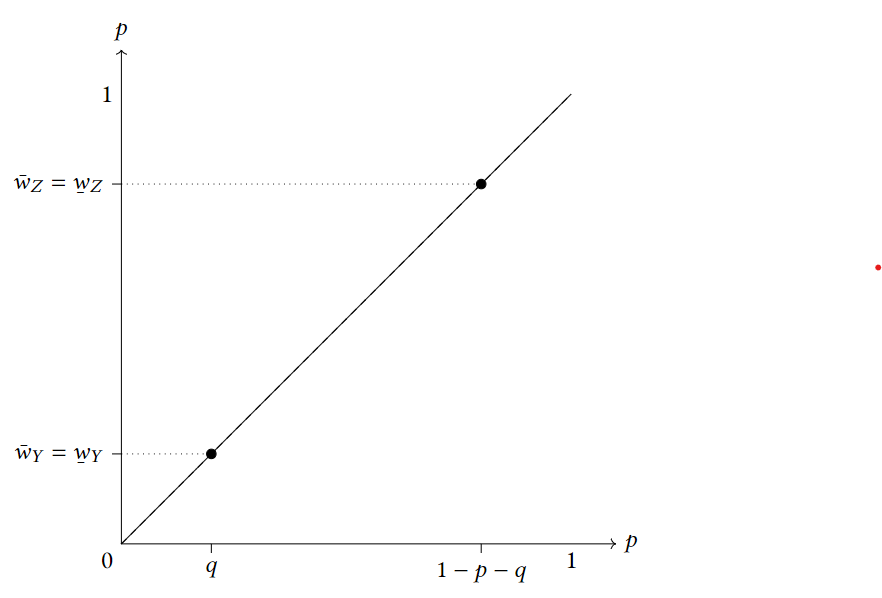
\includegraphics[width=1.4\linewidth,height=\textheight,keepaspectratio]{figures/EUWeights.png}

\begin{itemize}
\tightlist
\item
  EU predicts that weights are independent of \(X\)
\item
  Therefore, it predicts that \(k\) remains constant between \(\bar{L}\)
  and \(\underline{L}\)
\end{itemize}

\begin{center}\rule{0.5\linewidth}{0.5pt}\end{center}

\subsection{}\label{section-19}

\subsubsection{Equivalent variations allow tests for
rank-dependence}\label{equivalent-variations-allow-tests-for-rank-dependence-1}

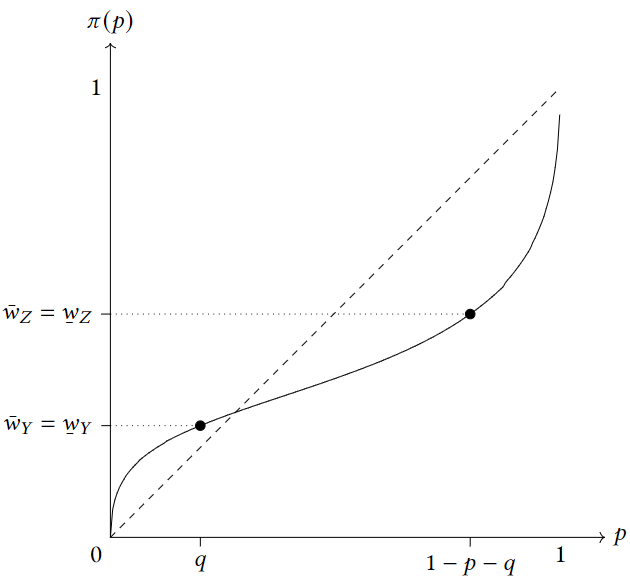
\includegraphics[width=0.95\linewidth,height=\textheight,keepaspectratio]{figures/PTWeights.png}

\begin{itemize}
\tightlist
\item
  Standard prob. weighting predicts that weights are independent of
  \(X\)
\item
  Therefore, it predicts that \(k\) remains constant between \(\bar{L}\)
  and \(\underline{L}\)
\end{itemize}

\begin{center}\rule{0.5\linewidth}{0.5pt}\end{center}

\subsection{}\label{section-20}

\subsubsection{Equivalent variations allow tests for
rank-dependence}\label{equivalent-variations-allow-tests-for-rank-dependence-2}

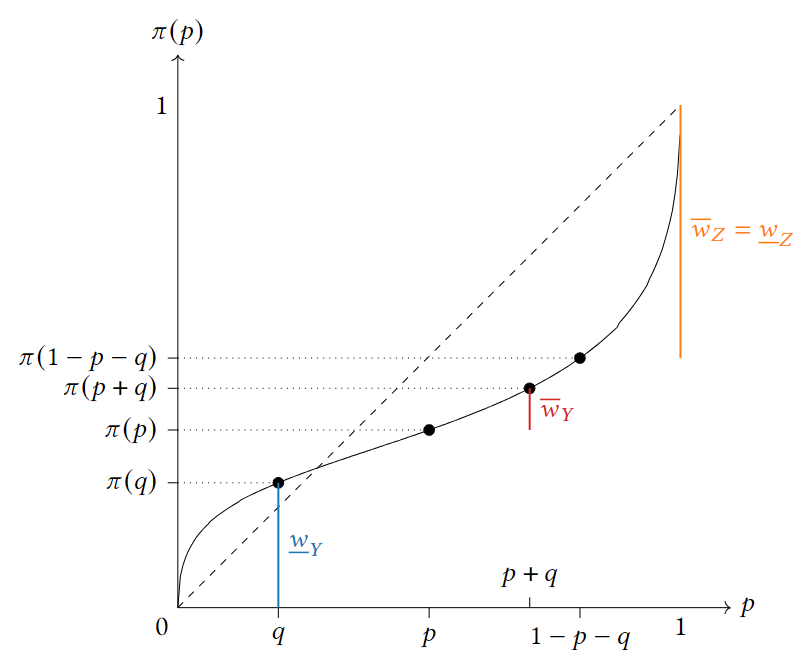
\includegraphics[width=1\linewidth,height=\textheight,keepaspectratio]{figures/CPTWeights.png}

\begin{itemize}
\tightlist
\item
  Rank-dependent prob. weighting predicts that weights are dependent on
  \(X\)
\item
  Therefore, it predicts that \(k\) changes between \(\bar{L}\) and
  \(\underline{L}\)
\end{itemize}

\begin{center}\rule{0.5\linewidth}{0.5pt}\end{center}

\subsubsection{Bernheim and Sprenger (ECTA, 2020): Prob. weights are
rank-independent}\label{bernheim-and-sprenger-ecta-2020-prob.-weights-are-rank-independent}

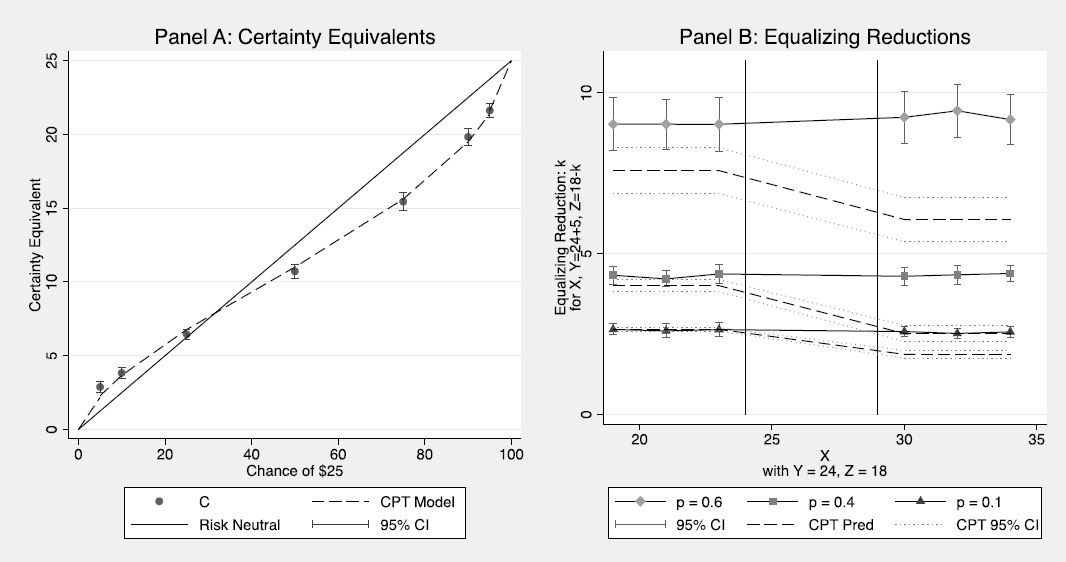
\includegraphics[width=0.6\linewidth,height=\textheight,keepaspectratio]{figures/CPTTest.png}

\begin{itemize}
\tightlist
\item
  Individuals weight probabilities (left panel).
\item
  Equivalent variations are independent of \(X\) (right panel)
  \(\rightarrow\) Weights are not rank-dependent
\end{itemize}

\begin{center}\rule{0.5\linewidth}{0.5pt}\end{center}

\subsection{Wrapping up}\label{wrapping-up}

\begin{itemize}
\tightlist
\item
  Classical theory: \(\text{EU / SEU + concave utility}\)
\item
  People deviate from the linear probability weighting prediction of EU
  / SEU
\item
  Probability weighting is better captured by \(\pi(p).\)
\item
  Risk attitutes: part preference, part a reaction to \emph{choice
  complexity}.
\item
  Non-linear prob. weighting leads to dominance violations, a
  theoretical solution exists but there is no empirical support for it.
\end{itemize}

\begin{center}\rule{0.5\linewidth}{0.5pt}\end{center}




\end{document}
